It is easy to see that a central piece of any platform security architecture is the security of OS kernel: any breach in this area almost always leads to the compromise of the whole system, especially if no security HW support is present. This makes the OS kernel a very attractive target and many recent studies show that adversaries are more and more focusing their efforts on kernel-level attacks~\cite{stoep2016android}.\todo[inline]{put more references} This is especially true given that many popular mobile and embedded OSes spent considerable effort in tightening the security of their userspace applications and processes~\cite{stoep2016android}.\todo[inline]{put more references} For example, it used to be pretty common that many userspace daemons run with superuser privileges all the time making it very easy for attackers to obtain these privileges straight after compromising a single userspace process. On the contrary nowadays the privileges of each userspace application or daemon are minimized, and higher privileges are quite commonly even limited to the system or daemon startup time: after the initialization phase is finished, unnecessary privileges are dropped and cannot be misused by an attacker if the process gets compromised later on. Another common improvement is compartmentalization and isolation of the most vulnerable application parts, such as parsers and renderers, into separate sandboxed processes further reducing attacker's opportunities. As a result of these efforts, modern successful attacks on userspace applications are very complex and require chaining of multiple vulnerabilities in order to reach the desired result. In contrast a single vulnerability directly in the OS kernel provides an attacker with superuser privileges right away.

This thesis focuses on a specific OS kernel, namely the Linux kernel, due to its widespread adoption for mobile and embedded devices: more than 2 billion mobile devices are currently running Android OS powered by the Linux kernel, many embedded manufacturers build their OSes based on Open Embedded/Yocto~\cite{OE2017, yocto2017} projects with the Linux kernel being at its base etc. 
In addition, the Linux kernel is developed fully in the open and any person is able to propose ideas or contribute the code to the mainline (of course given that the Linux kernel maintainers agree with the approach).

Past studies~\cite{stoep2016android, cooklss2016} show that the Linux kernel vulnerabilities have a remarkably long life time. It takes on average five years between the time when a vulnerability is introduced into the kernel source code and the time it is fixed. Moreover even after it is finally fixed in the mainline Linux kernel, it is very difficult to estimate when the fix is delivered to the end devices: it might take anything between a number of days to a number of years. In addition some older embedded or mobile devices might actually never see these updates, making them perfect attack targets. The study~\cite{Thomas2015} done back in 2015 showed that on average 87.7\% of Android devices are exposed to at least 11 known critical vulnerabilities including the ones for the Android OS kernel itself. The time window between the public announcement of kernel vulnerability and its fix (usually pretty fast) in the mainline kernel and the time the fix is propagated to most of the devices is the period of golden opportunity for many attackers: all the details about the vulnerability is known and sometimes even proof-of-concept exploit can be obtained.

As adversaries have been turning towards attacking the Linux kernel itself, security architects, researchers and engineers have been exploring various methods for its better protection. A lot of the effort has been put into improving the overall testing suites for the Linux kernel, various static and dynamic code checkers are also used regularly and automated. New tools, including better commit verification scripts are being developed to assist developers, better code review practices are established etc. However, it is unrealistic to assume that it would ever be possible to have all the bugs in the source code found and fixed even in the well-maintained mainline Linux kernel. The situation is even much worse for drivers and other non-mainline code developed by OEMs~\cite{stoep2016android}. Such code might get a very limited code review, little testing and be written under harsh time-to-market requirements making it a good place for introducing bugs and vulnerabilities.

An alternative approach that defenders can take is to consider how modern kernel exploits are written and try to eliminate all attack paths that helps exploit writers to succeed. This is exactly the path that the Kernel Self Protection Project (KSPP)~\cite{kspp} has taken. KSPP is an open community of developers and security experts that aims to develop new or adapt existing kernel hardening measures for the mainline Linux kernel. 

Figure~\ref{fig:exploit-steps} shows how a typical attack on the Linux kernel is performed. In Step 1 an attacker usually spends time to explore the target kernel offline in order to collect as much information about it as possible. This step is usually performed with high privileges and an attacker has a full access to the kernel memory layout, various debugging and tracing tools etc. Preventing this step is impossible due to the open nature of Linux operating system, but various protection methods can be employed to minimize the value of collected information. For example, Kernel Address Space Layout Randomization (KALSR)~\cite{cook2013} and other techniques such as GRKERNSEC\_RANDSTRUCT~\cite{randstruct2017} can make sure that every time a Linux kernel is loaded on the system, the memory location of many its components is randomized, and therefore an attacker cannot use the information collected during Step 1 to locate required kernel elements (modules, symbols, structures etc.) during the later steps of a run-time attack. 

\begin{figure}[t]
	\centering
		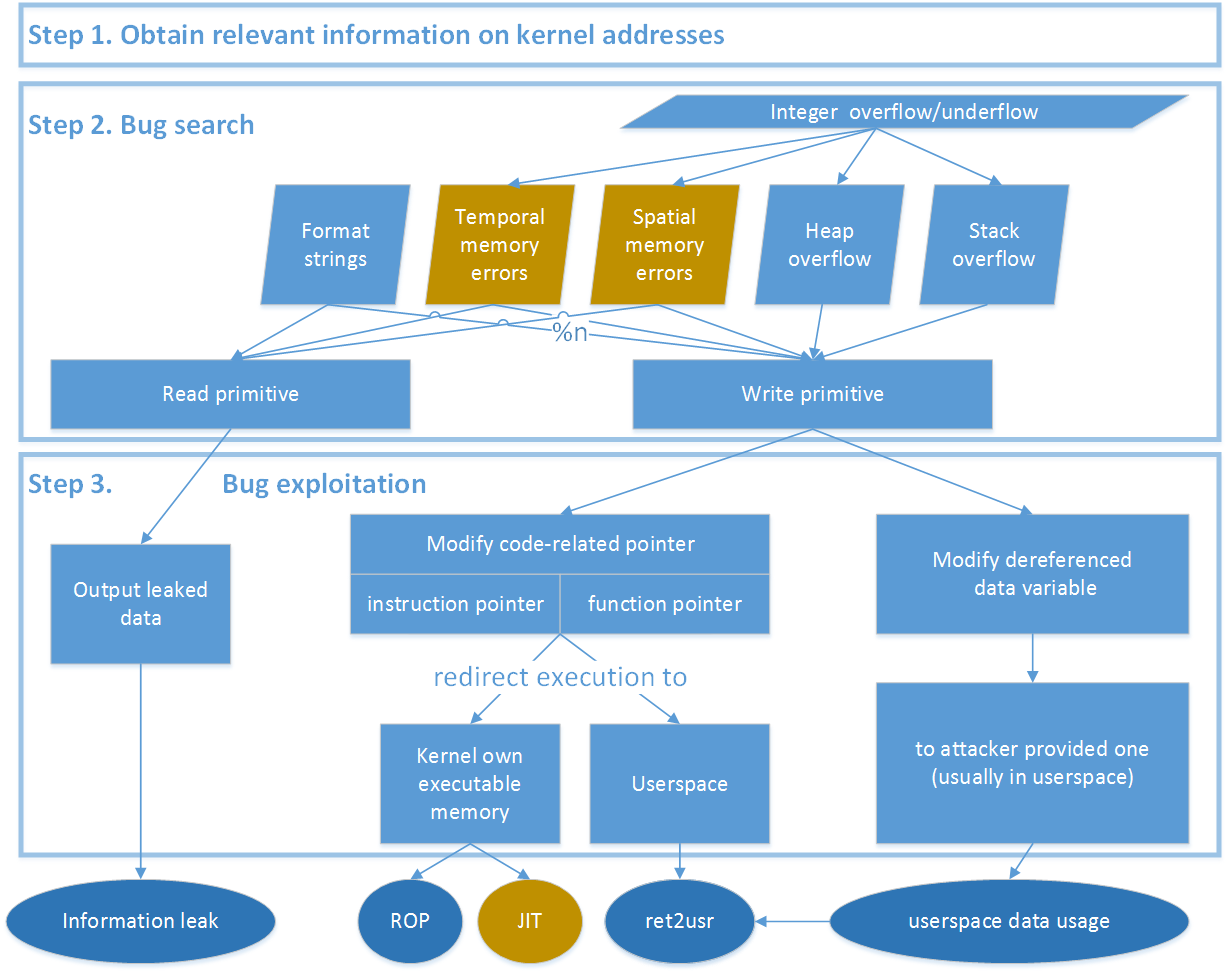
\includegraphics[width=1\textwidth]{figures/kernel_exploit_steps.png}
	\caption{High-level overview of a kernel attack}
	\label{fig:exploit-steps}
\end{figure}    

In Step 2 an attacker needs to find a suitable bug that would allow him to obtain a read or write primitive inside the Linux kernel. There are many bug classes that can be explored for this purpose with the most common ones being memory handling errors and stack/heap overflows\todo[inline]{put references}. Preventing Step 2 from happening would be an ideal case for defenders, but in reality it is very difficult and costly to prevent certain classes of bugs from fully happening. Nonetheless a lot of work is being done in this area within the KSPP project and Section~\ref{sec:kern-mem-safety} of this thesis looks into preventing a wide range of memory errors in the Linux kernel. 

Last in Step 3 an attacker can finalize the exploitation using the bug(s) found in Step 2. In case of a read primitive, the end result is usually a run-time kernel memory leak that can be either valuable on its own (various sensitive information, such as keys and credentials) or can be used as supporting information for launching further attack steps using another kernel bug. In turn, a write primitive can be used by an attacker to modify either a code-related pointer or a dereferencing of a kernel data pointer or structure. The code-related pointer can be either directly an instruction pointer (as it is the case with stack overflow attacks) or a function pointer located in places such as function pointer and descriptor tables. All of this would allow an attacker to redirect the execution flow to a desired place. That place can be either the kernel's own executable memory (by building and chaining the available attack gadgets in ROP-like technique or using mechanisms like just-in-time (JIT) compilers) or userspace (various \textit{ret2usr} attacks), where an attacker usually has more control over the memory layout and more mechanisms for continuing the attack and making it persistent over reboots. An attacker can also modify a data pointer (commonly to a structure located in the userspace) that might allow him to perform various data-only attacks. Many different protections can be put in place in order to prevent Step 3 from happening, but they are not generic and depend on the chosen attack path. For example in order to prevent a function pointer overwrite, function pointer tables can be made read-only after the kernel initialization step. Similarly in order to prevent a direct modification of an instruction stack pointer various return address protection techniques, such as stack canaries~\cite{edge2014}, guard pages~\cite{kstackoverflow2017} etc. can be employed.    

Within the KSPP project this thesis has investigated into two important areas of kernel hardening that are highlighted in orange in Figure~\ref{fig:exploit-steps}). The first one is preventing attackers from misusing the Berkeley Packet Filter (BPF) Just-In-Time (JIT) compiler in order to place the attack payload. The BPF JIT compiler is the only JIT compiler in the Linux kernel that executes programs supplied by unprivileged userspace, making it a very valuable target for the attackers.  The second area is an ability to prevent kernel memory errors, such as use-after-frees or buffer overflows, that can greatly affect the overall security of the Linux kernel and help eliminating many past and future vulnerabilities. The subsections below explain each aspect in more details as well as the contribution this thesis makes in addressing these two problem areas.  

\section{Security of Berkeley Packet Filter Just-In-Time compiler}
\label{sec:bpf-jit-attack}

Having an OS kernel mechanism with the ability to execute userspace-supplied code is always very attractive for attackers. 
The mainline Linux kernel has such mechanism: the Berkeley Packet Filter (BPF)~\cite{kernelfilter2016} and the associated Just-In-Time (JIT) compiler, that is basically an in-kernel virtual machine available for unprivileged execution from the userspace. Historically this mechanism was introduced to speed up packet filtering on networking sockets, but nowadays it is also used in a wide range of non-networking applications, including trace points~\cite{starovoitov2015}, syscalls filtering in seccomp~\cite{seccomp2016}, Kernel Connection Multiplexer (KCM)~\cite{corbet2015} etc. There is even a proposal to use BPF for creating a user-programmable Linux Security Module, Landlock~\cite{landlock2016}, that considerably widens the set of BPF use cases.

\begin{figure}[t]
	\centering
		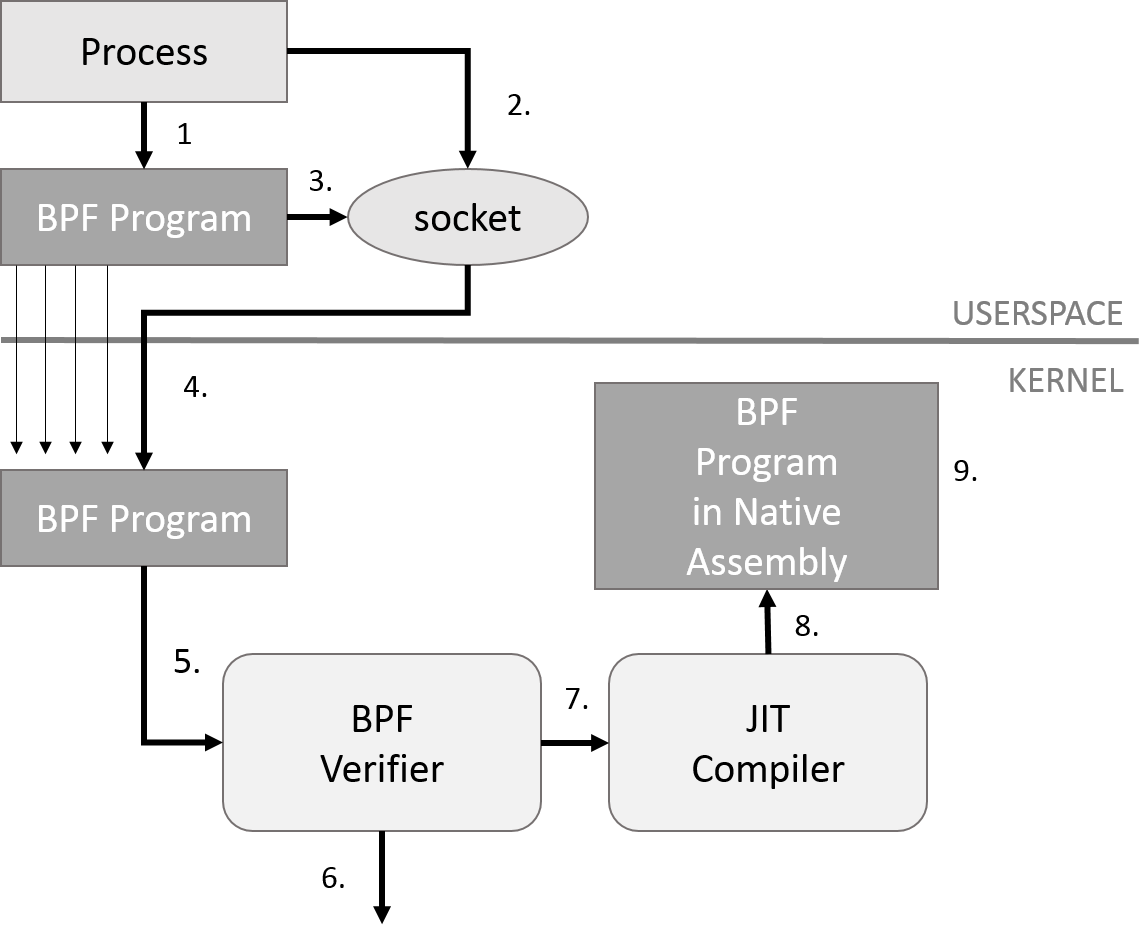
\includegraphics[width=0.80\textwidth]{figures/bpf-overview.png}
	\caption{Linux kernel Berkeley Packet Filter and JIT compiler (From Publication V)}
	\label{fig:bpf-overview}
\end{figure}

\todo[inline]{Remember to either get the copyright permission or modify the figure}          


The overall flow of how a BPF program is processed by the kernel is shown is shown in figure~\ref{fig:bpf-overview}.  
A userspace process expresses its packet filtering algorithm in a form of the BPF program that it wants to attach to a socket. A BPF program is written in the BPF interpreter language that can be executed by BPF in the kernel. When a BPF program is loaded to the kernel, it is first verified by a BPF Verifier component that attempts to check the correctness of supplied program. If the check passes, then the program is attached to the socket and will be executed every time the packet is received for that socket. However, in order to further speed up the filtering, the BPF program can be given to the JIT compiler that translates it to the native machine assembly language. 

The above flow can be abused to load the attacker-supplied payload into the kernel memory using an attack technique called \textit{JIT spraying}~\cite{blazakis2010, bania2010jit}. The original proof-of-concept exploit was done back in 2012~\cite{mcallister2012attacking} and showed that BPF JIT compiler design and implementation are very vulnerable to such attacks. As a result a protective measure was merged in the mainline kernel that attempted to randomize the start memory address where the BPF program gets loaded and insert the poisoned architecture-specific instructions before that address that would hang the machine fully if attacker tries to execute them. This made it really hard (with a probability of success only about 0.0004\%) for an attacker to find supplied payload. However, the root cause of the problem was not fixed at that time, despite the suggestions from some security experts\footnote{The Grsecurity kernel security project \url{grsecurity.net}}.

Publication V of this thesis analyzes the security issues of the BPF JIT compiler and builds a number of successful attacks on the latest at that time available mainline 4.4 Linux kernel despite the security fixes done in the past. 
Our best attack approach, described in Section 4.3 of publication V, analyzes how memory allocation for a BPF program happens and specifically how randomization of the start address is done in the mainline kernel implementation. This analysis discovered that for certain sizes of the BPF programs (size can be controlled by an attacker) the maximum size of the poisoned zone can be calculated in advance and it allows an attacker to reliably jump over the poisoned zone and land securely on the BPF program payload. The resulting overall success rate for the attack is 99.6\%, which proves that much stronger security measures are required for the BPF JIT compiler in order to provide an adequate security against JIT spray attacks. As a result of this work a number of mitigation measures were merged to the mainline kernel that fully eliminated possibility to perform this type of attacks\footnote{\url{git.kernel.org/cgit/linux/kernel/git/torvalds/linux.git/commit/?id=4f3446b}}. It is no longer possible to supply the attacker's payload in BPF programs using the constants due to the blinding process (XORing with a random number) done for each of them prior to its placement in the memory.

\section{Kernel memory safety}
\label{sec:kern-mem-safety}

Memory errors can be very dangerous for the security of OS kernel since they can give an attacker an ability to read or write kernel memory, which is normally inaccessible for a userspace process. The cause of these errors is an absence of inherent memory safety in C, which is the primary implementation language of the Linux kernel. 
Numerous past CVEs (CVE-2014-2851, CVE-2016-4558, CVE-2016-0728, CVE-2014-0196, CVE-2016-8440, CVE-2016-8459, and CVE-2017-7895) as well as vulnerability studies~\cite{raheja2016analysis, chen2011linux} show that memory errors is a big problem for the Linux kernel and needs addressing in order to be more robust against these attacks.

Typically memory errors are divided into two classes:

\begin{itemize}
	\item \textbf{Temporal memory errors}. These errors happen when pointers to uninitialized or freed memory are dereferenced. A typical example is a \emph{use-after-free} error when a dereferenced pointer has already been prematurely freed. Another example is a null pointer dereference errors, when an initialized pointer is attempt to being dereferenced. 
	\item \textbf{Spatial memory errors}. These errors occur when pointers are dereferenced outside the bounds of their intended areas. The most common example here is a buffer overflow when a data written past the end of memory allocated for the buffer. 
\end{itemize}

Overall the topic of memory safety has been researched for decades both in academia and industry.
Many solutions have been proposed to fully eliminate the root cause of the problem, but they are rarely used in practice due to the significant side effects they bring. 
The primary issue is usually the performance and most of the developed solutions~\cite{hastings1991purify},~\cite{patil1995efficient, patil1997low},~\cite{nagarakatte2009softbound},~\cite{jones1997backwards},~\cite{yong2003protecting, xu2004efficient, nethercote2004bounds}, and ~\cite{dhurjati2006backwards} incur a significant and non-acceptable run-time performance overhead.
Other typical issues are lack of backwards compatibility~\cite{necula2002ccured},~\cite{grossman2005cyclone},~\cite{austin1994efficient} and a need to make source code changes~\cite{necula2002ccured},~\cite{grossman2005cyclone}. 
In addition almost all existing mechanisms are developed for the userspace and have not been considered for in-kernel use with the exception of recently developed kCFI~\cite{Rigo} and KENALI~\cite{kenali}. However, even these systems have not been developed with the goal of merging them into the mainline Linux kernel and therefore exhibit some design choices that won't be acceptable by the mainline kernel developers\footnote{\url{http://www.openwall.com/lists/kernel-hardening/2017/08/05/1}}. 

Publication VI of this dissertation takes a deep look on both temporal and spatial memory problems in the Linux kernel and proposes two practical measures that address each of these types of errors. 

\subsection{Preventing temporal memory errors for objects protected by a reference counter}
\label{sec:kern-mem-ref-count}

A lifetime of a shared object in the Linux kernel is typically managed using a \textbfit{reference counter}. 
Such counter is incremented every time a reference to an object is taken and decremented when a reference is released. 
When the counter reaches zero the object can be safely deleted since there are no references to this object anymore (object is not used).

The above presents a simple logic, but practice and history of Linux kernel vulnerabilities (for example CVE-2014-2851, CVE-2016-4558, CVE-2016-0728, CVE-2017-7487 and CVE-2017-8925) shows that reference counting schemes are error prone. If a developer forgets to perform an increment or decrement on some code branch (quite often on a rarely exercised error handling or exception path), it might lead to counter imbalance and as a result incorrect object lifetime handling, i.e. use-after-free situation on the object. This can be misused by attackers in order to construct the efficient and simple kernel exploits. One such example is the exploit based on kernel CVE-2016-0728\footnote{\url{https://www.exploit-db.com/exploits/39277/}}. The exploit abuses a bug inside kernel keyring facility: forgotten decrement of the reference counter when substituting the session keyring with the same keyring. 
The problem is even bigger given the fact that the current implementation of reference counters in the Linux mainline kernel allows a counter to overflow upon reaching its maximum value (specific to the architecture). 

The first part of the publication VI analyzes how developers have used reference counters in the Linux kernel and contributes to the design of a new reference counter data type \setype{refcount\_t} and API that prevents reference counter overflows by its internal design. 
The new type is specifically designed for the reference counting use only and therefore has a much more limited API compare to the existing generic type, \setype{atomic\_t}, used for many other purposes. This allows to reduce the potential development errors when implementing reference counters and improves the code review process.   
This type and respective API have been accepted into the mainline Linux kernel and are becoming a de-facto standard for implementing reference counters. 
One of the biggest parts of the work was an overall kernel-wide analysis and conversion of existing reference counters to the newly available type and API that resulted into more than 170 accepted patches\todo[inline]{update exact number since it is changing all the time}. The analysis was done using a static analyzer, Coccinelle~\cite{coccinelle}, integrated into the Linux Kernel build system (KBuild). A set of code patterns was developed for this purpose that identify reference counters based on their behavior. These code patterns are explained in more details in Section 4.1 of the Publication VI. After the automatic analysis has been completed, each case was manually analyzed and a respective patch created. 


\subsection{Preventing out-of-bounds memory accesses}
\label{sec:kern-mem-out-of-bounds}

As was already mentioned in Section~\ref{sec:kern-mem-safety} none of the existing run-time mechanisms to handle memory access errors are directly applicable to the mainline Linux kernel. However other mechanisms are commonly used for the debugging purposes.
KASAN~\cite{kasan}, integrated in the mainline Linux kernel, is perhaps the most known of them all. It allows to detect a wide range of memory errors, including spatial ones. However its performance overhead is unsuitable for most production use cases.
Another examples include popular Valgrind~\cite{nethercote2007valgrind} and AddressSanitizer~\cite{serebryany2012addresssanitizer} tools. 

Recently Intel has released a new technology, \intel Memory Protection Extensions (MPX)~\cite{ramakesavan2015intel}, for an efficient run-time prevention of spatial memory errors that is targeting a wide range of end devices from desktops to mobile and embedded processors.  As many related solutions, MPX does it by determining (either during compile time or during the run-time) the correct bounds for each used pointer and storing this data in the separated metadata storage. Pointer bounds are enforced by MPX instrumentation using added hardware instructions, essentially by checking memory addresses before dereferencing pointers. The checks are done against bounds set by compiler instrumentation, either statically based on data structure sizes, or during execution by instrumented allocators. The above software support is implemented both in the Linux kernel and the GCC compiler, but until recently, this software support only worked for user-space applications. 
 
The second part of the publication VI analyzes the software implementation of \intel MPX as well as various challenges of using MPX for the Linux kernel itself. The major challenge was a high memory overhead incurred by the mechanism how MPX stores the bounds for the pointers. If such mechanism is directly applied to the Linux kernel, it would result in more than $500\%$ increase for the kernel base memory, which is unacceptable. The on-demand memory allocation mechanism for the userspace, used by MPX in attempt to minimize its memory consumption, is also not possible to implement reliably for the Linux kernel itself. Other challenges included an inability to use the MPX initialization code created for the userspace, userspace function wrappers, as well as the GCC compiler support directly for the kernel code.
As a result Publication VI proposes a new mechanism, \emph{MPX for Kernel (MPXK)}, which is an adaptation of \intel MPX for in-kernel use where all the above described challenges has been solved. MPXK does not use the costly memory storage mechanism of MPX, but instead re-uses the kernel memory management metadata created by \setype{kmalloc}-based allocators. This results in a small memory footprint, but has some limitations explained in details in Sections 5.1 and 6.1 of Publication VI. MPXK also implements all the missing GCC compiler instrumentation in a form of a new GCC plugin, as well as does in-kernel initialization of MPX and function wrappers to pass the bounds metadata. 

\section{Discussion}

In order to perform a high-level evaluation of the solutions proposed in this chapter and their impact on the researched area, it is important to start from the original objectives defined in Section~\ref{sec:Objectives}: security, practical deployability and usability. A more formal and detailed evaluation of solutions proposed in this chapter can be found in the evaluation sections of publications V and VI. 

The attacks described in Section~\ref{sec:bpf-jit-attack} built a strong case for the mainline acceptance of BPF JIT blinding protections that considerably improved security of Linux kernel BPF/JIT. Originally this attack was possible because the blinding solution developed by Grsecurity~\cite{grsecurity} was considered as an unnecessary complication to the BPF JIT functionality impacting code maintainability and performance. And since the only existing practical 2012 proof-of-concept exploit~\cite{mcallister2012attacking} could be stopped with a much simpler measures (start address randomization and poisoning zone), the constant blinding technique was not implemented in the mainline kernel until the work within the KSSP project on BPF/JIT has started. 

The measures to harden Linux kernel reference counters, described in Section~\ref{sec:kern-mem-ref-count}, aim to significantly decrease hard-to-find developers mistakes on reference counter usage and therefore prevent resulting use-after-free situations on shared kernel objects. If such measures would be in place in past, they would have prevented many kernel vulnerabilities mentioned in Section~\ref{sec:kern-mem-ref-count}. The newly introduced \setype{refcount\_t} type and API guarantee that a reference counter cannot overflow under all conditions, and our kernel-wide conversion of reference counters to this newly available type (175 from 220) provides a good initial code coverage with more and more conversions added in each kernel release. While the overall effectiveness of this measure would be only possible to judge with time, the proposed solution is also practically deployable and usable: it exhibits acceptable performance overhead for most of workloads, can be applied on case-by-case basis and it has been taken into use by its main intended users, kernel developers and maintainers. 

The MPXK mechanism, described in Section~\ref{sec:kern-mem-out-of-bounds}, aims to protect the Linux kernel from all spatial memory errors and therefore prevent a wide class of attacks caused by them. MPXK ensures that pointers to the objects with known bounds cannot be dereferenced outside of these bounds. However in some cases the correct bounds cannot be reliably determined and therefore MPXK has a number of limitations connected with usage of legacy code, type of memory allocation and some cases of direct pointer manipulations. The practical deployability of MPXK is judged based on a small performance overhead and an ability to apply the protection only in required places (with a compilation unit granularity) compared to the system-wide solutions like KASAN. MPXK does not require any source code changes and it is fully integrated into the Kernel build infrastructure making it easy for kernel developers to enable protection where required.  

